\documentclass{beamer}
\usepackage{graphicx} % Required for inserting images
\usepackage[OT1]{fontenc}
\usepackage{tikz}
\usetikzlibrary{positioning}


\title{Pares únicos de Fourier para as potências de inteiros}
\author{Afonso Vilhena Francisco}
\date{26 de Julho de 2026, Fundação Calouste Gulbenkian}

\setbeamertemplate{blocks}[rounded]
\setbeamercolor{block title}{bg=gray!15,fg=black}
\setbeamercolor{block body}{bg=gray!5,fg=black}


\begin{document}


\begin{frame}{}
    \titlepage
    $$\textbf{Tutor: } \text{Diogo Oliveira e Silva}$$

\end{frame}

\begin{frame}{}
    \textbf{Princípios de Incerteza}: Um princípio de incerteza afirma que determinadas características de um certo objeto matemático não são necessariamente independentes.


    \vspace{0.5cm}
    \pause
    \begin{block}{Transformada de Fourier}
        Definimos a transformada de Fourier de uma função de Schwartz $f: \mathbb{R} \rightarrow \mathbb{C}$ como
        $$\hat{f}(\xi)=\int_{\mathbb{R}}f(x)e^{-2\pi i x \xi }dx$$
    \end{block}

    \tiny Uma função diz-se de Schwartz se as derivadas de todas as ordens forem de decaimento rápido.
    No espaço de Schwartz, a transformada de Fourier é um automorfismo.
\end{frame}

\begin{frame}{}
    \begin{block}{Heisenberg (dezembro)}
        Se f é uma função de Schwartz tal que $\int_{\mathbb{R}}|f(x)|^2dx=1$, então
        $$\left( \int_\mathbb{R}x^2|f(x)|^2dx \right) \left(  \int_\mathbb{R}\xi^2|\hat{f}(\xi)|^2d\xi \right) \geq \frac{1}{16\pi^2}$$
    \end{block}
\vspace{0.8cm}
\pause
    \begin{block}{Hardy (dezembro e março)}
        Seja $f$ uma função de Schwartz tal que $f(x)=O(e^{-\pi Ax^2 })$ e $\hat{f}(\xi)=O(e^{-\pi B \xi^2})$, com $A,B >0$.
        Se:
        \begin{itemize}
            \item $AB=1$, então $f(x)=Ce^{-\pi Ax^2}$, com $C \in \mathbb{R}$
            \item $AB>1$, então $f \equiv 0$
        \end{itemize}
    \end{block}
\end{frame}

\begin{frame}
    \begin{block}{Pares únicos}
         Dada uma função de Schwartz $f: \mathbb{R} \rightarrow \mathbb{C}$, diz-se que  $A, \widehat{A} \subset \mathbb{R}$ é um \textbf{par único de Fourier} se a seguinte implicação é satisfeita 
    \[
    \begin{aligned}
        f(x) &= 0 \quad \text{para todo } x \in A\\
        \hat{f}(\xi) &= 0 \quad \text{para todo } \xi \in \widehat{A}
    \end{aligned}
    \quad \Rightarrow \quad
    f \equiv 0
    \]
    \end{block}

\end{frame}

\begin{frame}{Motivação}

    \begin{block}{Fórmula de Interpolação (Radchenko and Viazovska, 2017)}
        Existem funções de Schwartz pares $a_n $ tal que

        $$f(x)=\sum_{n=0}^\infty f(\sqrt n)a_n(x)+\sum_{n=0}^\infty \hat{f}(\sqrt{n})\hat{a_n}(x),$$

        qualquer que seja a função de Schwartz par $f:\mathbb{R} \rightarrow \mathbb{C}$.
    \end{block}
    {\tiny Uma fórmula semelhante vale para funções de Schwartz ímpares.}

    \vspace{0.5cm}
    
    \pause


    \begin{block}{Corolário}
        $A=\hat{A}=\{\pm n^{1/2}\}_{n \in \mathbb{N}}$ é um par único de Fourier.
    \end{block}

\end{frame}


\begin{frame}{}

\begin{block}{Problema:}
    Que condições devem satisfazer $\alpha$ e $\beta$ para que 
    $$A_\alpha := \{ \pm n^\alpha \}_{n \in \mathbb{N}} \text{ e } A_\beta:=\{ \pm n^\beta \}_{n \in \mathbb{N}} $$
    formem um par único de Fourier?
\end{block}

\vspace{0.5cm}
\pause

\begin{block}{Teorema (J.P.G.Ramos e M.Sousa, 2019)}
    Se 
        \[
        (\alpha,\beta)\in[0,1]^2,\qquad
        \alpha+\beta<1,
        \]
        
        e
        
        \[
        \alpha<1-\frac{\beta}{1-\alpha-\beta}
        \quad\text{ou}\quad
        \beta<1-\frac{\alpha}{1-\alpha-\beta},
        \]
            então $$(A_\alpha, A_\beta) \text{ é um par único de Fourier}.$$
\end{block}
\end{frame}

\begin{frame}{}
    \begin{block}{Corolário (Caso diagonal)}
        Para $\alpha<1-\frac{\sqrt{2}}{2} \approx 0.293$, $(A_\alpha,A_\alpha)$ é um par único de Fourier.
    \end{block}

\pause

\begin{figure}[H]
    \centering
    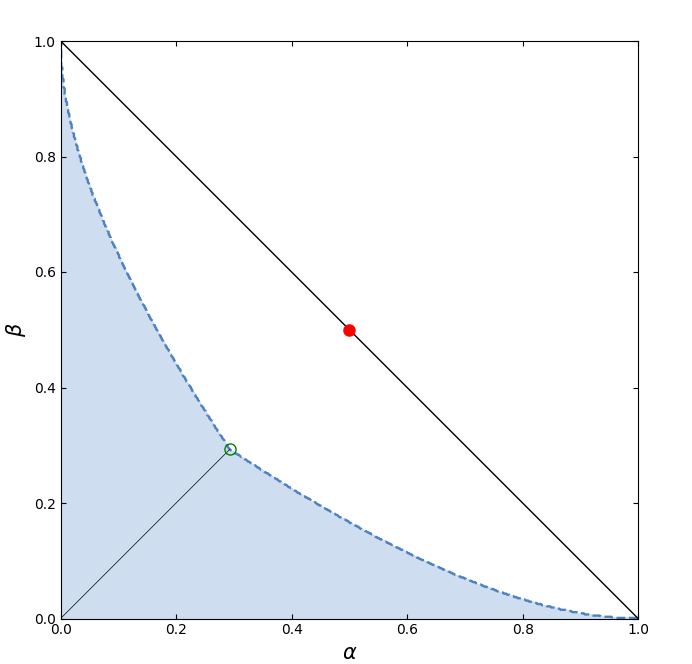
\includegraphics[width=0.7\linewidth]{fig1 (3).png}
\end{figure}

\end{frame} 

\begin{frame}{}
Seja $f \neq 0$ e  $L_1:=\frac{\alpha}{1-\alpha-\beta}$, $L_2:=\frac{\beta}{1-\alpha-\beta}$
\begin{center}
\resizebox{0.95\textwidth}{!}{
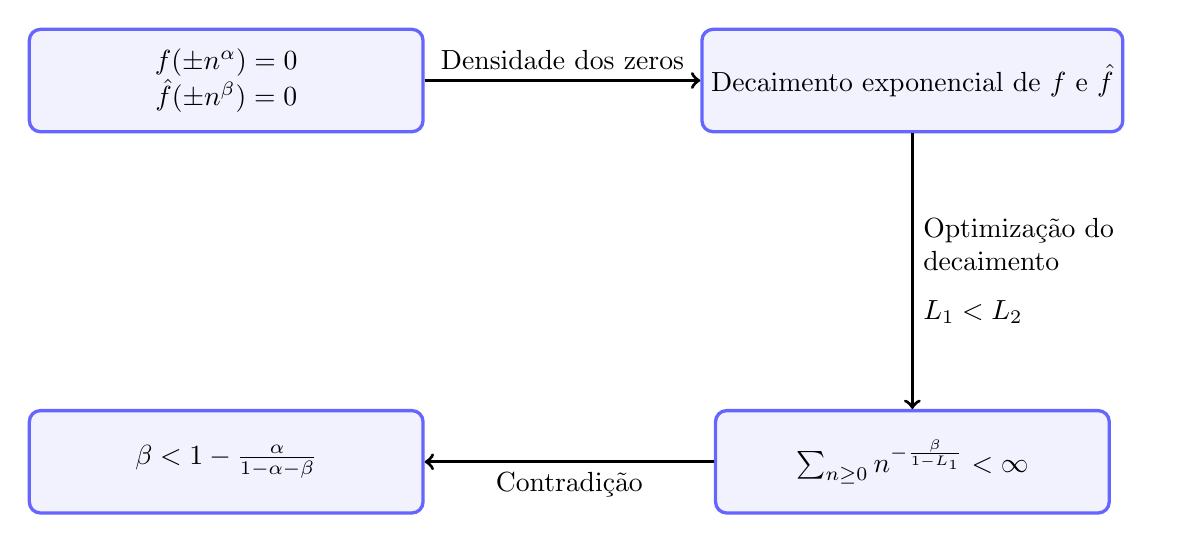
\begin{tikzpicture}[
    node distance=3.5cm,
    SIR/.style={
        rectangle, 
        draw=blue!60, 
        fill=blue!5, 
        very thick,
        rounded corners,
        minimum width=5cm,
        minimum height=1.3cm,
        align=center
    },
    arrow/.style={->, very thick}
]

\node[SIR] (A) 
{$f(\pm n^\alpha)=0$\\
$\hat{f}(\pm n^\beta)=0$};

\node[SIR] (B) [right=of A] 
{Decaimento exponencial de $f$ e $\hat{f}$};

\node[SIR] (C) [below=of B] 
{$\sum_{n \geq 0} n^{-\frac{\beta}{1-L_1}} < \infty$};

\node[SIR] (D) [below=of A] 
{$\beta<1-\frac{\alpha}{1-\alpha-\beta}$};

\draw[arrow] (A) -- node[above] {Densidade dos zeros } (B);
\draw[arrow] (B) -- node[
    right,
    align=left,
    text width=3cm
]{
Optimização do decaimento\\[2mm]
$L_1<L_2$
} (C);Contradição
\draw[arrow] (C) -- node[below] {Contradição } (D);

\end{tikzpicture}
}
\end{center}
\end{frame}

\begin{frame}{}
    \begin{block}{Pares supercríticos e subcríticos}
        Sejam $\Lambda=(\lambda_j)_{j \in \mathbb{Z}}$ e $M=(\mu_j)_{j \in \mathbb{Z}}$ sucessões crescentes ilimitadas por cima e por baixo.

        Dados $1<p,q<\infty$ com $\frac{1}{p}+\frac{1}{q}=1$, dizemos que o par $(\Lambda, M)$ é 

        \begin{itemize}
            \item supercrítico se
            $$\limsup_{|j| \rightarrow \infty} |\lambda_j|^{p-1}(\lambda_{j+1}-\lambda_j)<\frac{1}{2} \;\text{ e }\; \limsup_{|j| \rightarrow \infty} |\mu_j|^{q-1}(\mu_{j+1}-\mu_j)<\frac{1}{2}$$

            \item subcrítico se
            $$ \limsup_{|j| \rightarrow \infty} |\lambda_j|^{p-1}(\lambda_{j+1}-\lambda_j)>\frac{1}{2} \;\text{ e }\; \limsup_{|j| \rightarrow \infty} |\mu_j|^{q-1}(\mu_{j+1}-\mu_j)>\frac{1}{2}$$
        \end{itemize}
        
    \end{block}

    \pause

    \begin{block}{Teorema (A.Kulikov, F.Nazarov e M.Sodin, 2023)}
        Qualquer par supercrítico é um par único de Fourier.\\
        Qualquer par subcrítico não é um par único de Fourier.
    \end{block}

\end{frame}


\begin{frame}{}

\begin{block}{Corolário}
    Seja $(\alpha,\beta)\in[0,1]^2$. Se 
    \begin{itemize}
        \item $\alpha+\beta<1$, então $(A_\alpha, A_\beta)$ é um par único de Fourier.
        \item $\alpha +\beta>1$, então $(A_\alpha, A_\beta)$ não é um par único de Fourier.
    \end{itemize}
\end{block}
\pause

\begin{figure}[H]
    \centering
    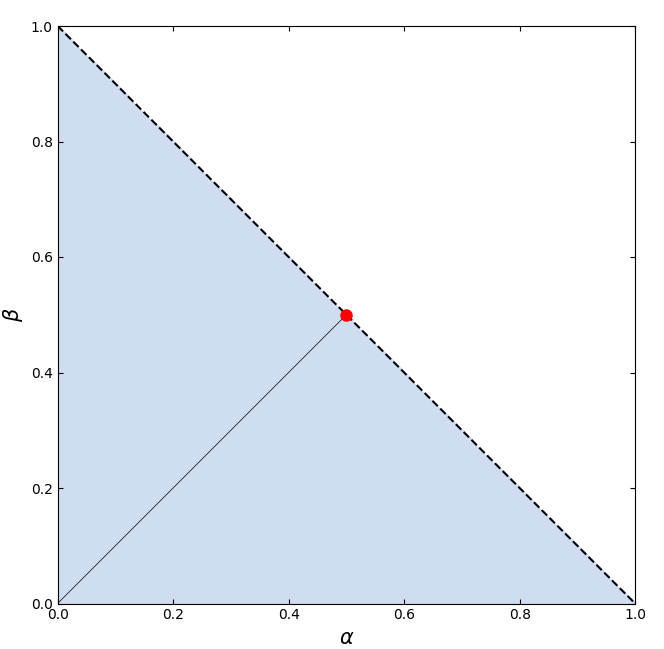
\includegraphics[width=0.6\linewidth]{fig2 (1).png}
\end{figure}

\end{frame}

\begin{frame}{}
    \Large $$\text{ Próximos Passos }$$
    \Large $$\text{ e }$$
    \Large $$\text{ Reflexão Pessoal }$$
\end{frame}

\begin{frame}{}
\Large $$\text{Obrigado pela vossa atenção!}$$
\end{frame}

\begin{frame}{}
\begin{block}{Passo 1}
Escolher $$(\lambda_n)_{n \in \mathbb{N}}=(\pm n^\alpha)_{n \in \mathbb{N}} \text{ e } (\mu_n)_{n \in \mathbb{N}}=(\pm n^\beta)_{n \in \mathbb{N}}$$
\end{block}
\pause
\begin{block}{Passo 2}
    \begin{align*}
        \lim_{n \rightarrow \infty}\lambda_n^{p-1}(\lambda_{n+1}-\lambda_n)&=\alpha \lim_{n \rightarrow \infty}(n^{\alpha p-1})
    \end{align*}

        \begin{align*}
        \lim_{n \rightarrow \infty}\mu_n^{q-1}(\mu_{n+1}-\mu_n)&=\beta \lim_{n \rightarrow \infty}(n^{\beta q-1})
    \end{align*}

\end{block}    
\pause
\begin{block}{Passo 3}
    Como $\alpha + \beta <1$, podemos escolher $p,q$ tal que $$\frac{1}{p}+\frac{1}{q}=1 \;\text{ e }\; \alpha p<1, \,\beta q<1$$ 
\end{block}
\end{frame}

\end{document}
